\section{Ausblick}

\begin{quotation}
"`Die Welt ist voller Fragen. Aber jede Frage schlie�t eine Hoffnung in sich ein."' - Hans Margolius \cite[S. 27]{Ansorg_2008}
\end{quotation}

Die vorliegende Arbeit wurde in der Hoffnung verfasst, einen Teil zur L�\-sung des Problems um Gewaltdarstellungen in
Computerspielen beitragen zu k�nnen. Die schwierigste Aufgabe bei der Suche nach Antworten ist, zuerst die richtigen
Fragen zu stellen. W�hrend sich die Forschung bisher eher auf die Frage nach der Wirkung von Gewalt in Computerspielen
konzentrierte, lag der Entwicklung von Cydonia die Frage nach ihrer Notwendigkeit zugrunde.\par


\subsection{Die n�chsten Schritte}
Damit das Konzept von Cydonia Erfolg haben kann, muss aus dem Prototypen ein fertiges Spiel werden. Viele Details wurden
bei der Entwicklung schlicht aus Zeitgr�nden vernachl�ssigt. Der Fokus lag auf der Untersuchung des gewaltfreien
Konzepts und seiner Elemente. Passende Ava\-tar\-mo\-del\-le, Equipment-Modelle, Animationen, Men�s, individualisierbare
Steuerung, detaillierte Ansicht der verf�gbaren Server, In-Game-Chat oder Ping-Anzeige stellen nur einige der Dinge dar,
die noch realisiert werden m�ssten. Wie in Abschnitt \ref{subsubsection:Netcode} bereits erw�hnt, ist der Netzcode nur
grundlegend implementiert und m�sste stark optimiert werden, vor allem wenn Cydonia auch �ber das Internet gespielt
werden soll.

\subsection{Offene Fragen}
Jede Antwort wirft auch wieder neue Fragen auf. Die Spieler, die den ersten Prototypen getestet haben (vgl. dazu
\ref{subsection:UsabilityTests}), hatten alle bereits im Voraus Erfahrungen mit dem Spielen von Shootern gesammelt. Eine
Folgestudie k�nnte beispielsweise untersuchen, ob Spieler, die die in Kapitel \ref{section:CaseStudy} beschriebene
direkte Einwirkung auf den Gegner nicht bereits kennengelernt haben, im Vergleich zu Shooter-erfahrenen Spielern
positiver auf ein Spiel reagieren, das keine solche direkte Einwirkung erm�glicht.\par In weiteren Studien k�nnte
au�erdem das Ph�nomen des Zweikampfes, das in Kapitel \ref{section:CaseStudy} betrachtet wurde, noch detaillierter
analysiert werden. Unter Einbeziehung m�glichst vieler Beispiele, bei denen Zweikampf-Si\-tua\-tionen auftreten, k�nnten
evtl. erg�nzende gewaltfreie Umsetzungen des Prinzips der direkten Einwirkung auf den Gegenspieler entwickelt werden.\\

Ist es gelungen, Shooter-Spieler mit einem gewaltfreien Spiel zu �ber\-zeu\-gen? Diese Frage kann bisher nur teilweise
beantwortet werden. Der Prototyp ist noch nicht ausgereift genug, um es mit anderen Spielen auf dem Markt aufzunehmen.
Auch hatte erst eine kleine Auswahl von Spielern die Gelegenheit, Cydonia zu testen. Doch die ersten Versuche zeigen,
dass es sich lohnt, den eingeschlagenen Weg weiter zu gehen.

\begin{figure}[htbp]
\centering
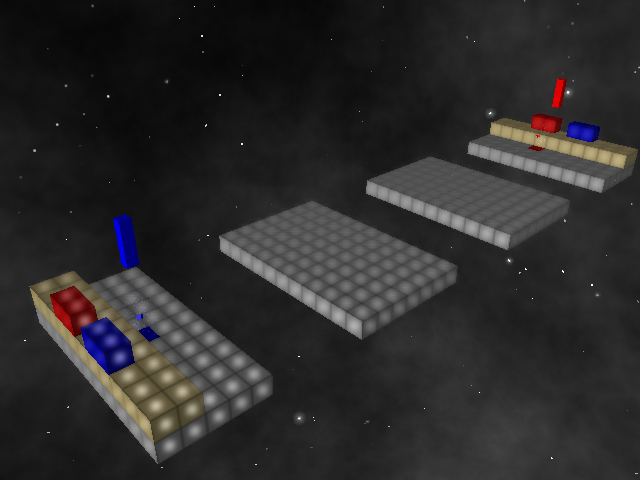
\includegraphics[width=0.8\textwidth]{images/screenshot_3}
\caption[Screenshot von Cydonia: �berblick �ber eine Spielwelt]{Screenshot von Cydonia: �berblick �ber eine Spielwelt}
\label{figure:screenshot_3}
\end{figure}